% Preamble:
% \usepackage{tikz}

\begin{figure}[ht]
\centering
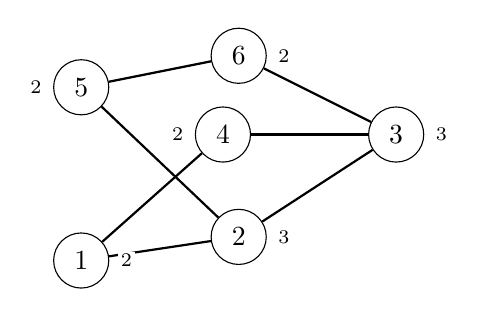
\begin{tikzpicture}[
  v/.style={circle, draw, minimum size=7mm},
  e/.style={thick},
  deg/.style={font=\scriptsize, fill=white, inner sep=1pt}
]
% --- 6 vertices (placed "randomly") ---
\node[v] (1) at (0,0)   {$1$};
\node[v] (2) at (2,0.3) {$2$};
\node[v] (3) at (4,1.6) {$3$};
\node[v] (4) at (1.8,1.6) {$4$};
\node[v] (5) at (0,2.2) {$5$};
\node[v] (6) at (2.0,2.6) {$6$};

% --- edges (no edge labels) ---
\draw[e] (1)--(2);
\draw[e] (2)--(3);
\draw[e] (3)--(4);
\draw[e] (4)--(1);
\draw[e] (2)--(5);
\draw[e] (5)--(6);
\draw[e] (3)--(6);

% --- degree annotations d(v) next to each vertex ---
\node[deg, anchor=west] at ([xshift=3pt]1.east) {$2$};
\node[deg, anchor=west] at ([xshift=3pt]2.east) {$3$};
\node[deg, anchor=west] at ([xshift=3pt]3.east) {$3$};
\node[deg, anchor=east] at ([xshift=-3pt]4.west) {$2$};
\node[deg, anchor=east] at ([xshift=-3pt]5.west) {$2$};
\node[deg, anchor=west] at ([xshift=3pt]6.east) {$2$};

\end{tikzpicture}

\caption{A simple undirected graph on $V=\{1,2,3,4,5,6\}$ with vertex degrees shown.
For example, $d(2)=3$ because vertex $2$ is adjacent to $\{1,3,5\}$, while $d(1)=2$ because vertex $1$ is adjacent to $\{2,4\}$.}
\label{fig:degrees-example}
\end{figure}
